\SECTION{Evaluation}
\label{sec:evaluation}
The runtime overhead and real-time performance of Linux-RTXG was evaluated.
The runtime overhead is classified into interrupt interception, independent synchronization, and priority-driven scheduling in Linux.
It is demonstrated in the following that the overhead of the LKM-based real-time scheduler for GPU applications is acceptable.
The real-time performance is verified in terms of QoS management and prioritization using both synthetic workload and real-world applications on top of three different device drivers, namely, NVIDIA, Nouveau, and Gdev.
It is also demonstrated that multiple GPU applications co-scheduled by the LKM-based real-time scheduler are successfully prioritized and maintained at the desired frame rate even under high CPU load.

Given that CPU scheduling performance has already been demonstrated in a previous work~\cite{kato2009loadable}, only GPU scheduling performance was experimentally evaluated in this work.
Considering the results of this work and those from the previous work, it is clarified that both emerging GPU applications and traditional CPU applications can be scheduled according to priorities and resource reserves by using LKMs, without modifying the Linux kernel and device drivers.

\SUBSECTION{Experimental Setup}
Experiments were conducted using the Linux kernel 3.16.0, an NVIDIA GeForce GTX680 GPU, a 3.
40-GHz Intel Core i7 2600 (eight cores including two hyperthreadling cores), and 8-GB main memory.
GPU application programs were written in CUDA and compiled by NVCC v6.0.1. A NVIDIA 331.62 driver and a Nouveau Linux-3.16.0 driver with NVIDIA CUDA 6.0 and Gdev were used.

\SUBSECTION{Interrupt-interception Overhead} 
The overhead incurred by interrupt interception was measured by using the Nouveau GPU driver to quantify the overhead of interception in the case of varied interrupt types.
As performance metrics, elapsed time from the beginning to the end of the ISR was adopted.


\begin{figure*}[!t]
\begin{minipage}[t]{0.33\hsize}
\begin{center}
\raisebox{-3mm}{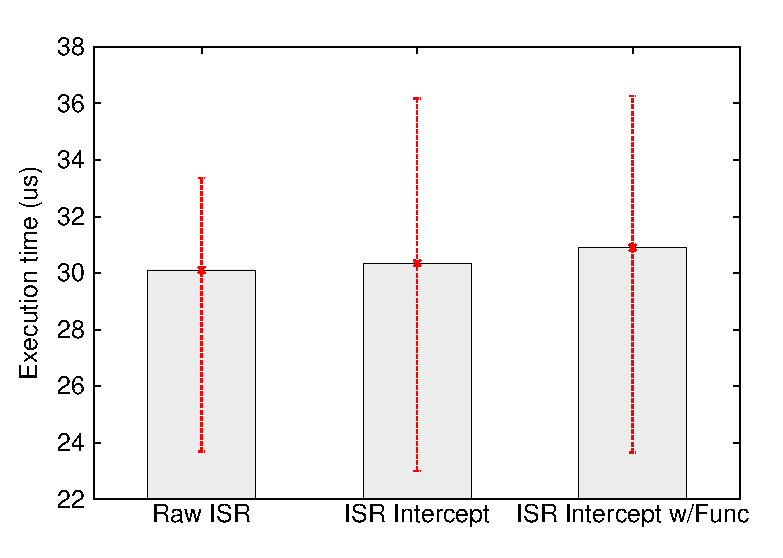
\includegraphics[width=62mm]{img/interrupt}}
\end{center}
\caption{\small{Interrupt interception overhead. \newline \,}}
\label{fig:irq_overhead}
\end{minipage}
\begin{minipage}[t]{0.33\hsize}
\begin{center}
\raisebox{-1mm}{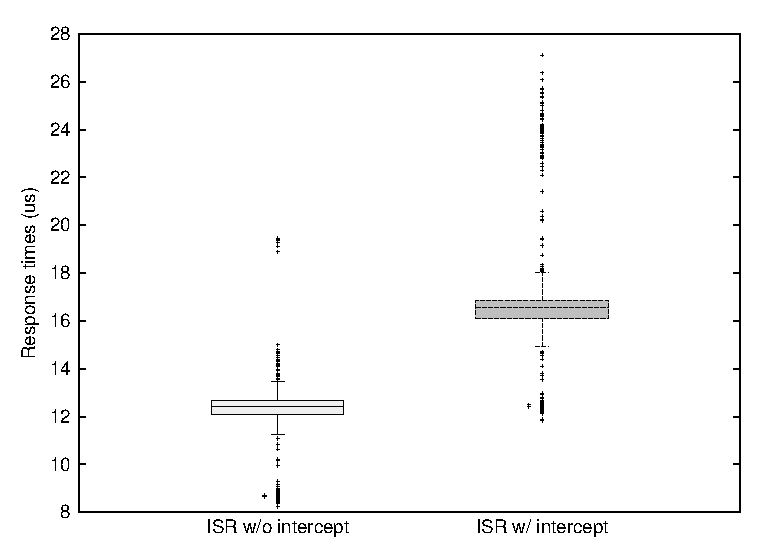
\includegraphics[width=62mm]{img/interrupt_response}}
\end{center}
\caption{\small{Impact of interrupt interception.}}
\label{fig:response}
\end{minipage}
\begin{minipage}[t]{0.33\hsize}
\begin{center}
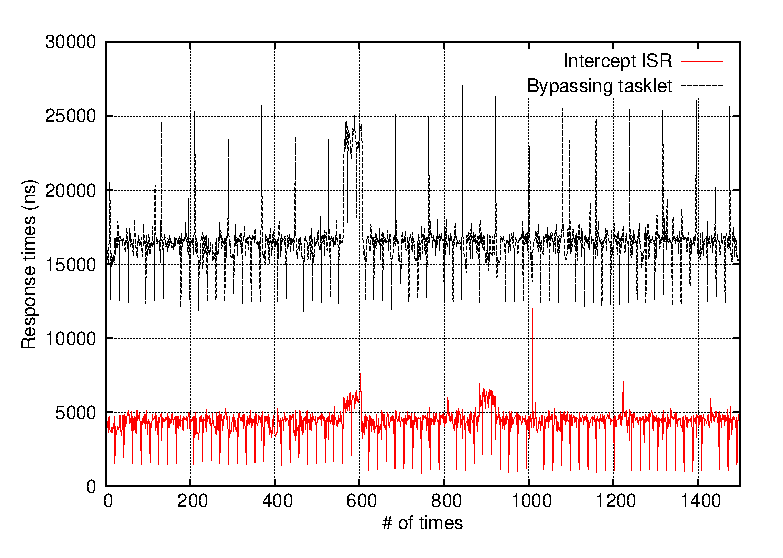
\includegraphics[width=62mm]{img/tasklet_vs_interrupt}
\end{center}
\caption{\small{Comparison of ISR and tasklet.}}
\label{fig:bottomvstasklet}
\end{minipage}
\end{figure*}

The overhead for interrupt interception is shown in Figure~\ref{fig:irq_overhead}. ``Raw ISR'' represents the original implementation of ISR.
``ISR Intercept'' represents the modified ISR with the interrupt interception mechanism, while ``ISR Intercept w/Func'' includes the overhead for identifying the ISR and calling the scheduler thread in addition to ``ISR Intercept''.
The average execution time for 1000 executions is presented with error bars.


Comparing Raw ISR and ISR Intercept indicates that the overhead for introducing the interrupt-interception mechanism was $247ns$, which is only $0.
8\%$ of Raw ISR.
 Similarly, the overhead for introducing ISR Intercept w/Func was $790ns$, which is only $2.
6\%$ of Raw ISR.
 This result indicates that the interrupt-interception overhead is insignificant in regard to total performance.


As shown in Figure~\ref{fig:response}, response times of ISR with and without interrupt interception are compared next.
The response time is defined as the elapsed time from the beginning of interrupt processing to the point where the interrupt type (e.
g.
, timer, compute, FIFO, and GPIO) is identified.
According to the result, interrupt interception makes response times 1.4-times longer.

Response times when interrupt interception is self-contained in the ISR (top-half) and when it is expanded to the tasklet (bottom-half) were also compared.
This comparison differentiates Linux-RTXG from GPUSync in terms of performance, since GPUSync intercepts the $tasklet\_schedule()$ on top of the proprietary driver, while Linux-RTXG realized ISR-based interception.
In this case, the start time of measuring the response time is set to that of the function call to $do\_IRQ$.
The result of this comparison is shown in Figure~\ref{fig:bottomvstasklet}.
As can be seen from this figure, the tasklet-based approach requires about five-times longer response times than the IRQ-based approach.
This is because the tasklet is typically called after significant ISR processing steps.


\SUBSECTION{Independent-synchronization Overhead}
The overhead of the independent synchronization mechanism was quantified next.
This mechanism must call $rtx\_gpu\_notify()$ at the time of requested synchronization (e.
g.
, after launching a GPU kernel).
To use this mechanism, an initialization procedure is required.
In this measurement, the overhead is defined by the execution time of corresponding APIs.


\begin{figure}[!t]
\begin{center}
\subfigure[Overhead for initialization]
{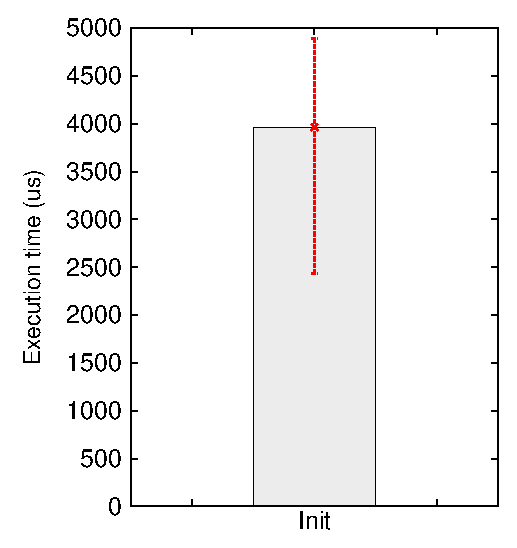
\includegraphics[width=0.23\textwidth]{img/irq_rise_init.eps}}
\subfigure[Overhead for notification]
{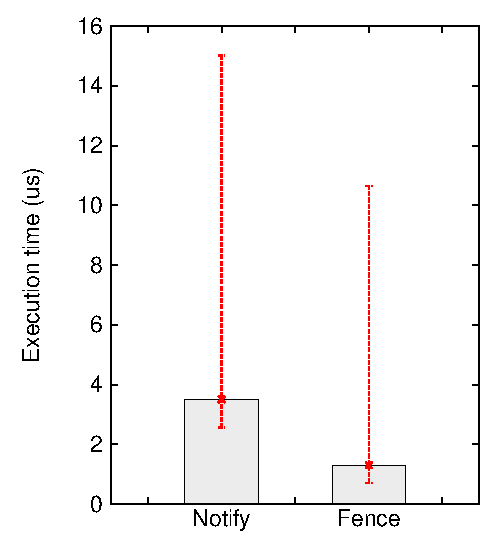
\includegraphics[width=0.22\textwidth]{img/irq_rise_notify.eps}}
\caption{Overhead for independent synchronization.}
\vspace{-4mm}
\label{fig:irq_rise_overhead}
\end{center}
\end{figure}

As shown in Figure~\ref{fig:irq_rise_overhead}, the initialization overhead could reach 5000$us$, whereas the notification overhead is no more than a few microseconds.
The initialization procedure calls a Linux process to allocate indirect buffers and control registers for several GPU engines.
Albeit a significant overhead, the application program is not much affected by this procedure, since it is called only once at the beginning.
On the other hand, the notification overhead is not a major consideration for the application program, though it is a little scattered due to an ioctl system call.
When NOTIFY is used to set notification, the overhead was $3.5us$, while it was reduced to $2us$ when FENCE is used.

\SUBSECTION{Scheduling Overhead}
\label{sec:eval:sched_overhead}

\begin{figure}[!t]
\begin{center}
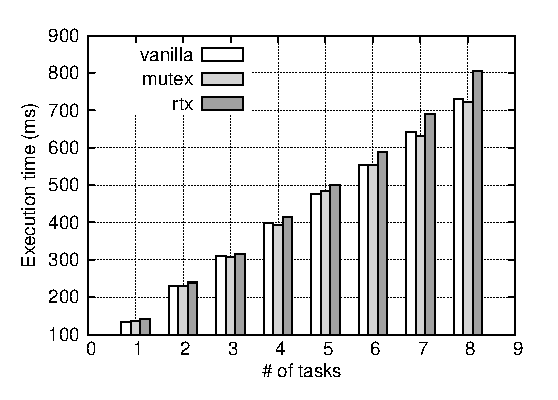
\includegraphics[width=.44\textwidth]{img/sum_task.eps}
\caption{Scheduling overhead.}
\vspace{-4mm}
\label{fig:fp_task_overhead}
\end{center}
\end{figure}

The scheduling overhead incurred by the presented Linux-RTXG scheduler was evaluated next.
Three synthetic tasks -- (i) vanilla, (ii) mutex, and (iii) rtx -- to measure the overhead were executed.
These tasks are based on the microbenchmark program provided by the Gdev project, which tests a GPU loop function.
The program was modified to generate multiple GPU tasks by using the $fork()$ system call.
Each task releases a job ten times periodically, each of which includes data transfer between the CPU and the GPU, followed by execution of the GPU kernel.
The rtx task was scheduled by Linux-RTXG.
The mutex task was limited to a single GPU kernel by using explicit mutual-exclusion control similar to the rtx task.
The vanilla task was not changed from the original microbenchmark program.
The CPU scheduling policy was set to $SCHED\_FIFO$, while the GPU scheduling policy was based on fixed priorities with GPU-resource reservation, called the BAND scheduling policy~\cite{kato:gdev}.
The independent synchronization mechanism is employed with NOTIFY.

Average time in 100 times of GPU task execution (1000 jobs) We measured.
The result is provided in Figure~\ref{fig:fp_task_overhead}.
The scheduling overhead increases in proportion as the number of tasks, because the time consumed in queueing GPU tasks is increased.
The maximum overhead corresponds to $10\%$ of the vanilla task for eight tasks.

\SUBSECTION{Prioritization and QoS Performance}
Experiments were also performed to evaluate prioritization and QoS performance for GPU applications provided by Linux-RTXG.
These performances of Linux-RTXG were evaluated on both the proprietary driver (NVIDIA) and the open-source driver (Nouveau), as compared to the built-in-kernel approach (Gdev).


\begin{figure*}[!t]
\begin{minipage}[t]{0.33\hsize}
\begin{center}
\subfigure[{\small FIFO on NVIDIA}]
{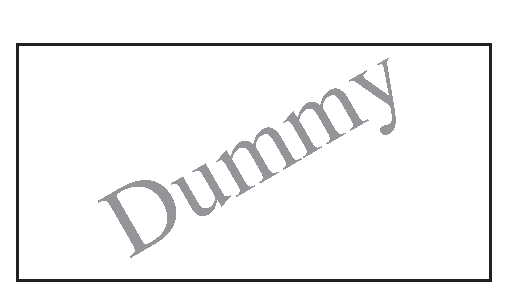
\includegraphics[width=62mm]{img/fifo_rtx_nvidia}} 
\label{fig:fifo_rtx_nvidia} \\
\subfigure[{\small BAND on NVIDIA}
]{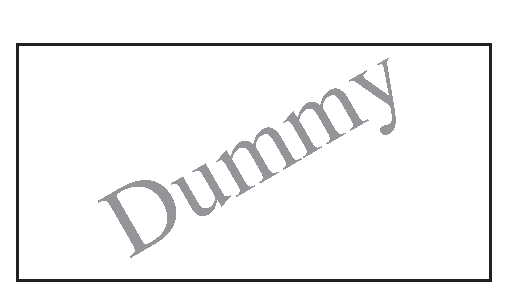
\includegraphics[width=62mm]{img/band_rtx_nvidia}}
\label{fig:band_rtx_nvidia}
\label{fig:rtx_nvidia}
\end{center}
\end{minipage}
\begin{minipage}[t]{0.33\hsize}
\begin{center}
\subfigure[{\small FIFO on Nouveau}]
{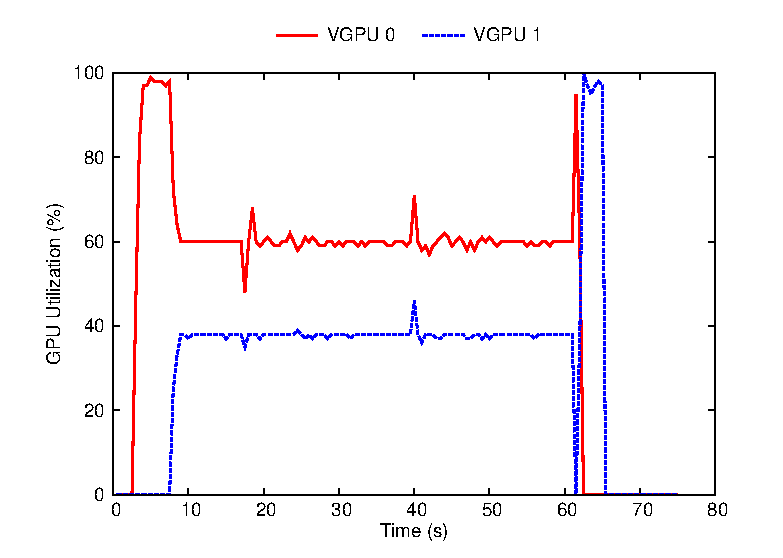
\includegraphics[width=62mm]{img/fifo_rtx}}
\label{fig:fifo_rtx} \\
\subfigure[{\small BAND on Nouveau}]
{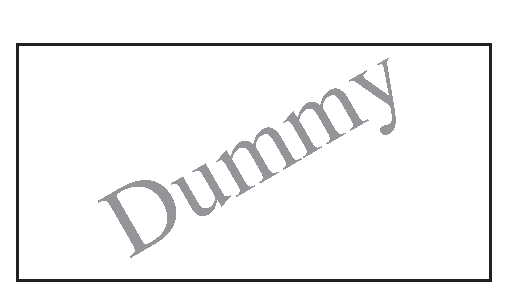
\includegraphics[width=62mm]{img/band_rtx}}
\label{fig:band_rtx}
\label{fig:rtx_nouveau}
\end{center}
\end{minipage}
\begin{minipage}[t]{0.33\hsize}
\begin{center}
\subfigure[{\small FIFO on Gdev}]
{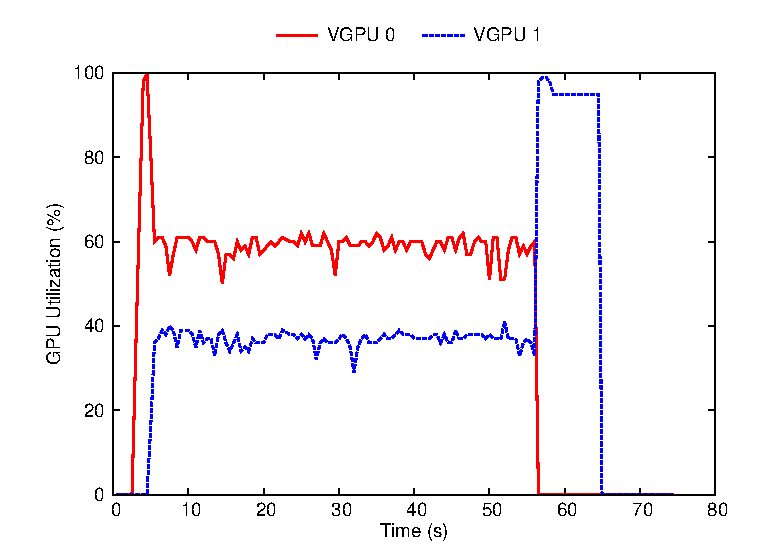
\includegraphics[width=62mm]{img/fifo_gdev}}
\label{fig:fifo_gdev} \\
\subfigure[{\small BAND on Gdev}]
{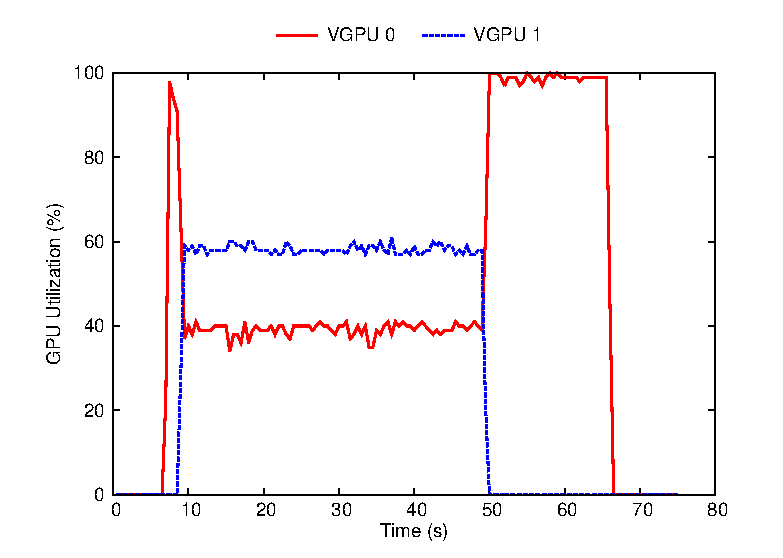
\includegraphics[width=62mm]{img/band_gdev}}
\label{fig:band_gdev}
\label{fig:gdev_usage}
\end{center}
\end{minipage}
\caption{GPU utilization of two tasks. Each task executes different types of GPU-intensive workloads with specified GPU reserves (VGPU0 = 40\%; VGPU1 = 60\%).}
\vspace{-3mm}
\label{fig:utilize}
\end{figure*}

\begin{figure}[!t]
\begin{center}
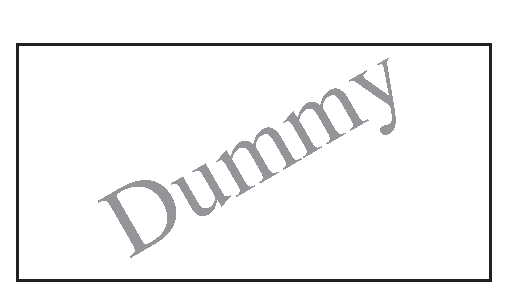
\includegraphics[width=0.4\textwidth]{img/band_rtx_fair}
\caption{Utilization of four tasks with the Linux-RTXG's BAND VGPU scheduling. Each task had an equal workload and an equal GPU-resource allocation.}
\vspace{-4mm}
\label{fig:band_rtx_fair}
\end{center}
\end{figure}

QoS management indicates if GPU time of the corresponding task is guaranteed.
QoS performance was evaluated by observing how well the tasks are isolated.
First, GPU utilization when running two GPU tasks was measured.
Each GPU task has a unique workload with a different size of GPU reserve.
One task was allocated to VGPU0, and given $40\%$ of GPU reserve.
This task (with a high priority) has $1.2$ times higher workload than the other, which was allocated to VGPU1 with $60\%$ of GPU reserve.
The VGPU1 task was scheduled to start approximately $5s$ after the VGPU0 task.


The result obtained under the FIFO scheduling policy on the NVIDIA Driver is shown in Figure~\ref{fig:utilize} (a), while that under the BAND scheduling policy is shown in Figure~\ref{fig:utilize}(b).
The corresponding results on the Nouveau GPU driver are shown in Figures~\ref{fig:utilize} (c) and (d).


Since VGPU0 has higher workload than VGPU1, the GPU tasks are performed in accordance with their workload, as shown in Figures~\ref{fig:utilize} (a) and (c).
On the other hand, the GPU resource-reservation mechanism provided by Linux-RTXG can successfully perform the GPU tasks in accordance with their reserves as indicated in Figures~\ref{fig:utilize} (b) and (d).
It is important to note that these prioritization and resource reservations for GPU applications can be achieved without modifying the OS kernel and device drivers in Linux-RTXG.


The maximum error of the VGPU1 task was approximately $3\%$ under the BAND scheduling policy on the NVIDIA driver, while that of the VGPU0 task was approximately $5\%$.
When the Nouveau driver was used, those values were $2\%$ and $6\%$, respectively.
These large increases occurred due to GPU kernel overruns.


In addition to the performance of the proposed loadable-kernel approach, the performance was compared with that of a prior work, Gdev.
The Gdev scheduling results are shown in Figures~\ref{fig:utilize} (e) and (f).
Almost no performance loss is imposed on Linux-RTXG as compared to Gdev.
In detail, when the Gdev scheduler was used, the maximum error of the VGPU1 task was approximately $3\%$ under the BAND scheduling policy, while that of the VGPU0 task was $5\%$.
There is also a large variation on a time basis when the Gdev scheduler was used.
This is because the runtime functions of Gdev must be called in the kernel space, where other system calls can easily block their operation.


GPU utilization running four GPU tasks was measured next.
Each GPU task has the same workload and the same GPU reserve on a different VGPU.
The isolation result for this scenario is shown in Figure~\ref{fig:band_rtx_fair}.
The maximum error of VGPUs was at most 9\%, which is incurred due to the timing of budget replenishment and synchronization latency.
In fact, this result almost matches that reported in a previous work on Gdev~\cite{kato:gdev} using the built-in kernel approach.
As a result, the independent-synchronization mechanism employed in Linux-RTXG does not sacrifice scheduling performance.


\begin{figure*}[!t]
\begin{minipage}[t]{0.33\hsize}
\begin{center}
\subfigure[{\small NULL.}]
{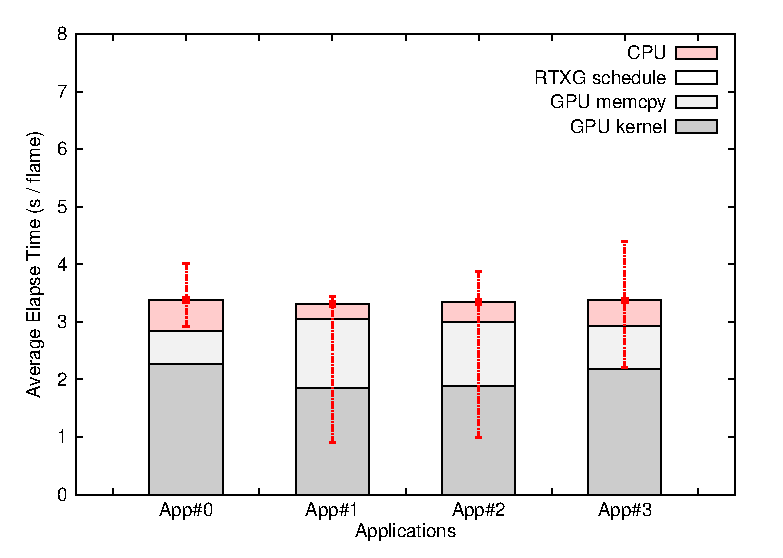
\includegraphics[width=62mm]{img/real_null_null_withoutload}}
\label{fig:real-null_null}
\subfigure[{\small FP.}]
{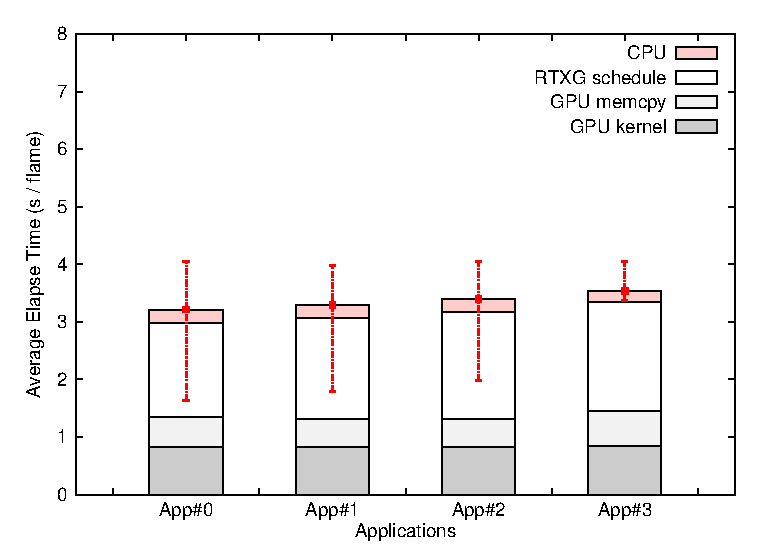
\includegraphics[width=62mm]{img/real_prio_null_withoutload}}
\label{fig:real-prio_null}
\end{center}
\end{minipage}
\begin{minipage}[t]{0.33\hsize}
\begin{center}
\subfigure[{\small BAND.}]
{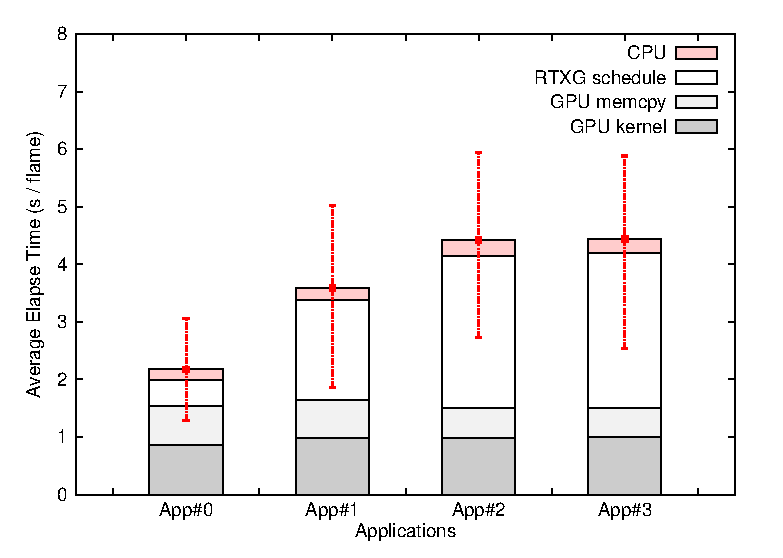
\includegraphics[width=62mm]{img/real_prio_band_withoutload}}
\label{fig:real-prio_band}
\subfigure[{\small BAND with high CPU load.}]
{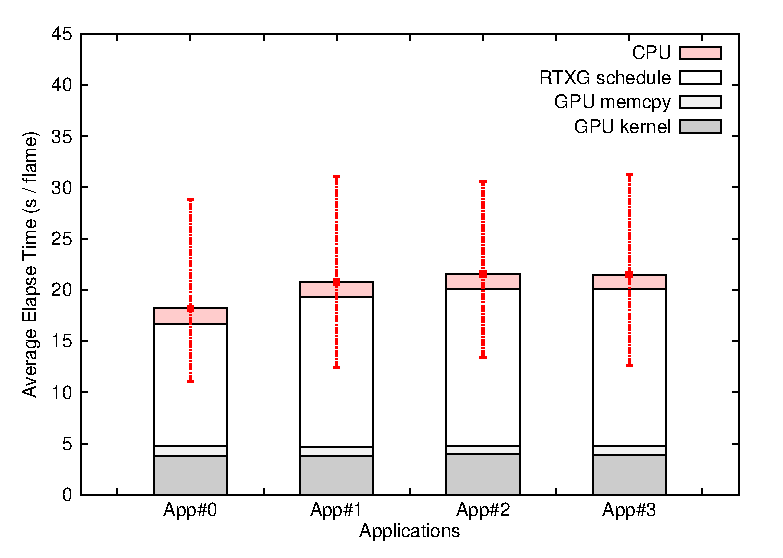
\includegraphics[width=62mm]{img/real_prio_band_withhighload}}
\label{fig:real-prio_band-hiload}
\end{center}
\end{minipage}
\begin{minipage}[t]{0.33\hsize}
\begin{center}
\subfigure[{\small NULL with high CPU load.}]
{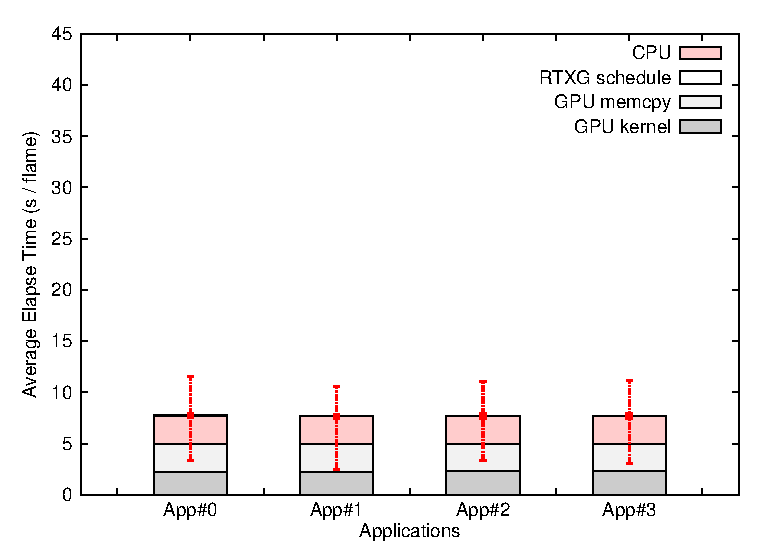
\includegraphics[width=62mm]{img/real_null_null_withhiload}}
\label{fig:real-null_null-hiload}
\subfigure[{\small FP and BAND with high CPU loads.}]
{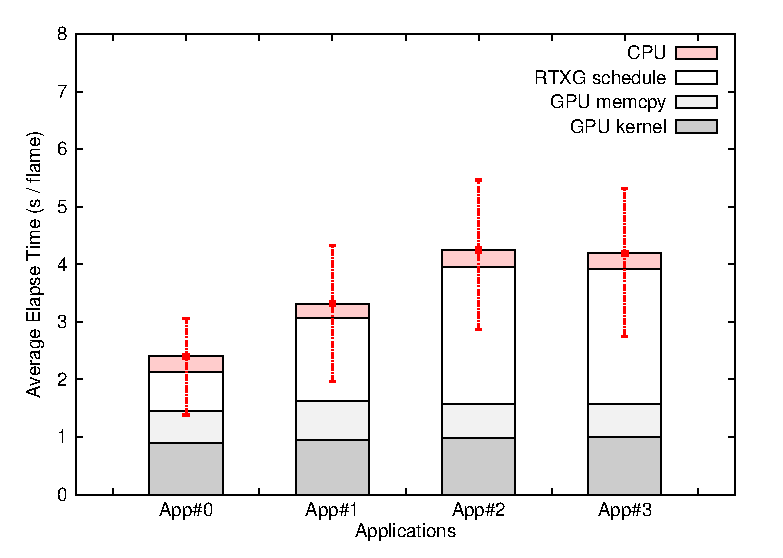
\includegraphics[width=62mm]{img/real_prio_band_withhighload_cpu}}
\label{fig:real-prio_band_cpu-hiload}
\end{center}
\end{minipage}
\caption{Execution time of the GPU-accelerated object-detection program.}
\vspace{-4mm}
\label{fig:elapse_time_all}
\end{figure*}

\SUBSECTION{Real-world Application}
The performance of Linux-RTXG on a real-world application was demonstrated as follows.
The demonstration was done with a GPU-accelerated object-detection program~\cite{hirabayashi:cpsna2013} based on the well-known DPM and HOG algorithms.
It was assumed that the monitoring system covered the four directions of the compass (east, west, south, and north).

The execution time per frame was measured in six different setups, as shown in Figure~\ref{fig:elapse_time_all}, where (a) no scheduling was applied, (b) fixed priorities were applied with GPU scheduling, (c) GPU resource reservation was further applied with the BAND scheduling policy, and (d), (e), and (f) high CPU load was contending with the $SCHED\_OTHER$ hackbench task.
The GPU tasks were allocated with $60\%$, $20\%$, $10\%$, and $10\%$ of GPU reserves, respectively.

The results of this experiment indicate that if a high-CPU load task exists, the performance of GPU tasks could be seriously affected, since GPU tasks cannot acquire CPU time needed to execute the GPU API.
Linux-RTXG can provide both CPU scheduling and GPU scheduling with resource-reservation capabilities to solve this problem, as shown in Figure~\ref{fig:elapse_time_all} (f).
As seen in the figure, the target programs are not affected by the high-CPU-load task thanks to the $SCHED\_FIFO$ scheduling, while GPU execution can be maintained at the desired frame rate thanks to the GPU-scheduling and resource-reservation capabilities.
These results demonstrate that Linux-RTXG can supply prioritization and QoS performance to real-world applications.
 

